\documentclass[12pt,twoside]{article}

% La extensión total de la memoria deberá ser de un máximo de 50 páginas (excluidos resumen, índice y posibles anexos).

% Según las recomendaciones de estilo, el formato de la memoria se ajustará a lo siguiente:
% ? Formato del papel: DIN A4.
% ? Impresión a dos caras.
% ? Márgenes: superior e inferior, 2.5 cm. Márgenes laterales: páginas impares, izquierdo 4 cm y derecho 2 cm; páginas % pares, izquierdo 2 cm y derecho 4 cm.
% ? Tipo de letra: Times New Roman de 12 puntos.
% ? Interlineado: 1.5 líneas.
% ? Alineación: justificación completa.
% ? Sangrado de párrafo: 0.5 cm la primera línea de cada párrafo. No se
%pondrá espacio entre párrafos.
% ? Las páginas deberán ir numeradas en números arábigos.

% Teniendo en cuenta las indicaciones previas, definimos el estilo en LaTeX:

% Indicaciones para el idioma:
\usepackage[T1]{fontenc}
\usepackage[utf8]{inputenc}
\usepackage[spanish]{babel}

% Adaptación de itemize y enumerate a los usos tipograficos españoles:
\let\layoutspanish\relax
\addto\captionsspanish{\def\tablename{Tabla}} % para que escriba "Tabla" en lugar de "Cuadro"
\unaccentedoperators  % para que no acentúe los operadores

% Área de impresión de una página:
\usepackage[a4paper]{geometry}
  \geometry{hmargin={2.5cm,2.5cm},height=22cm}

% Formato de algunas distancias:
\renewcommand{\baselinestretch}{1.2}    % separación entre líneas de un mismo párrafo
\setlength{\partopsep}{0pt}
\setlength{\itemsep}{0pt}
\setlength{\topsep}{0pt}
\setlength{\parsep}{0pt}
\setlength{\parskip}{0.25\baselineskip}   % separación entre párrafos

\renewcommand{\textfraction}{0.1}   % mínima fracción de la página para el texto
\renewcommand{\topfraction}{1}      % máxima fracción de la página para objetos flotantes en la parte superior
\renewcommand{\bottomfraction}{1}
\renewcommand{\floatpagefraction}{1}

\setcounter{totalnumber}{5}
\setcounter{topnumber}{3}
\setcounter{bottomnumber}{2}

% Adaptación de las "caption" de los entorns "figure" y "table":
\usepackage{caption}
\setcaptionwidth{\textwidth}
\addtolength{\captionwidth}{-2\parindent}
\captionsetup{margin=\leftmargini,%
  width=\captionwidth,%
  labelfont={up,bf},%
  font={small,sl},%
  %indention={\captionindent
}

% Indentación del primer párrafo de una sección:
\usepackage{indentfirst}

% Definición del color grisclaro en la salida PDF:
\usepackage[pdftex]{color}

% Gráficos:
\usepackage[pdftex]{graphicx}

% Paquetes recomendados para la inclusión de fórmulas matemáticas:
\usepackage{amsmath}
\allowdisplaybreaks  % para que pueda partir fórmulas que ocupan más de una línea, necesita el paquete anterior
\usepackage{amssymb} % para cargar algunos símbolos como \blacksquare y \square
\usepackage{amsfonts} % para cargar algunas fuentes en estilo matemático
\usepackage{enumerate}
% Teoremas (se pueden definir todos los que se necesiten):


\newtheorem{theorem}{Teorema}[section]
\newtheorem{proposition}[theorem]{Proposición}
\newtheorem{definition}[theorem]{Definición}
\newtheorem{lemma}[theorem]{Lema}
\newtheorem{corollary}[theorem]{Corolario}
\newtheorem{example}[theorem]{Ejemplo}
\newtheorem{app}[theorem]{Aplicación}
\newtheorem{remark}[theorem]{Observación}
\newtheorem{agrad}[theorem]{Agradecimiento}
\newtheorem{algo}[theorem]{Algoritmo}
\newtheorem{axiom}[theorem]{Axioma}
\newtheorem{case}[theorem]{Caso}
\newtheorem{conclu}[theorem]{Conclusión}
\newtheorem{conjectura}[theorem]{Conjetura}
\newtheorem{notac}[theorem]{Notación}
\newtheorem{soluc}[theorem]{Solución}
\newtheorem{summary}[theorem]{Sumario}

\newtheorem{proof}[theorem]{Demostración.}
\renewenvironment{proof}{\textbf{\emph{Demostración.}}} {\quad \hfill $\blacksquare$ \newline} % para que aparezca un cuadrado negro al acabar la demostración


% Definición de cabeceras y pies de página:

\usepackage{fancyhdr}                     % para definir distintos tipos de cabeceras y pies de página

\newcommand{\RunningAuthor}{Adán Avilés Cahill}
\newcommand{\Author}[1]{\renewcommand{\RunningAuthor}{#1}}
\renewcommand{\leftmark}{\RunningAuthor}

\newcommand{\RunningTitle}{Hacking Ético}
\newcommand{\Title}[1]{\renewcommand{\RunningTitle}{#1}}
\renewcommand{\rightmark}{\RunningTitle}


\pagestyle{fancy}
\fancyhf{}
\fancyhead[LO]{\small \slshape \leftmark}    % lo que aparece en la parte izquierda de la páginas impares
\fancyhead[RE]{\small \slshape \rightmark}   % lo que aparece en la parte derecha de las páginas pares
\fancyhead[RO,LE]{\small \slshape \thepage}  % el número de página aparece en la parte exterior de la cabecera

\renewcommand{\headrulewidth}{0.6pt}         % grueso de la línea horizontal por debajo de la cabecera de la página
\renewcommand{\footrulewidth}{0pt}           % grueso de la línea horizontal por encima del pie de página
                                             % en este caso está vacío
\setlength{\headheight}{1.5\headheight}      % aumenta la altura de la cabecera en una parte y media

\fancypagestyle{plain}{%                     % redefinición del estilo de página 'plain'
  \fancyhf{}                                 % limpia todas las cabeceras y pies de página
  \setlength{\headwidth}{\textwidth}
  \fancyfoot[C]{\small \slshape \thepage}    % excepto el centro del pie de página
  \renewcommand{\headrulewidth}{0pt}
  \renewcommand{\footrulewidth}{0pt}
  }

% Instrucciones que se usan frecuentemente
\newcommand{\abs}[1]{\ensuremath{|#1|}}
\newcommand{\norm}[1]{\left\lVert#1\right\rVert} %norma
\newcommand{\normd}[1]{\left\lVert#1\right\rVert_{2}} %norma
\newcommand{\hil}{\mathcal{H} }
\newcommand{\prodes}[2]{\langle #1, #2 \rangle }
\newcommand{\suc}{\{x_n\}_{n=1}^{\infty}}
\newcommand{\sumi}[2]{\sum_{#1}^{#2}}
\newcommand{\luno}{L^1(\mathbb{R})}
\newcommand{\ldos}{L^2(\mathbb{R})}
\newcommand{\tf}[3]{\dfrac{1}{\sqrt{2 \pi}} \int_{-\infty}^{\infty} #1 e^{-iw#2}d#3}
\newcommand{\erre}{\mathbb{R}}
\newcommand{\intif}{ \int_{-\infty}^{\infty}}
\newcommand{\cdos}{\mathcal{C}_{00}^{2} (\mathbb{R}) }
\newcommand{\tfd}{\mathcal{F}}

% Datos del trabajo y autor:
\title{Práctica Hacking Ético}
\author{Adán Avilés Cahill\\*[1em]
\begin{minipage}{0.75\textwidth}
\footnotesize \itshape
\begin{center}
IMF BUSINESS SCHOOL\\
Máster en Ciberseguridad
\end{center}
\end{minipage}
}
\date{Junio 2014}

% Para incluir paginas de otro pdf (por ejemplo, la de la portada):
\usepackage{pdfpages}

\setlength{\abovedisplayskip}{5pt}
\setlength{\belowdisplayskip}{5pt}

\pagestyle{fancy}
%----------------------------------------------------------------------------------
%-                                  DOCUMENT START                                -
%----------------------------------------------------------------------------------
\begin{document}
\begin{figure}[t]
 \begin{picture}(140,50) \put(140,0){
\includegraphics[width=60mm]{./imagenes/logo-imf-alta}} \end{picture}
\end{figure}

\title{Tecnologías SIEM}
\author{Adán Avilés}
\date{Julio 2020}
\maketitle


% A continuación, se incluirá el índice del trabajo y, seguidamente, se desarrollará la memoria.
\newpage
\tableofcontents
\newpage

% -------------------------------------------------% -------------------------------------------------
% -------------------------------------------------% -------------------------------------------------
% -------------------------------------------------% -------------------------------------------------
\section{Presentación y resolución de los problemas}
\subsubsection*{Durante el curso, hemos visto qué son los eventos correlados y los agregados. ¿Podría definir brevemente cada uno de ellos? Emplee gráficos, dibujos, ejemplos, etc., si lo cree oportuno.}

En primer lugar, definiremos lo que entendemos por \textbf{evento}. Un evento es todo registro que ha sido generado en una fuente de datos, la cual contiene información sobre las tareas y acciones realizadas por el sistema. Dependiendo de la aplicación o sistema que genere el evento, este será creado en un formato u otro, dependiendo de la aplicación.\\

Hablaremos de correlación cuando tengamos correspondencia o relación entre dos o más cosas, o series de cosas. Así, un motor de correlación es una aplicación software que entiende las relaciones de forma programática. Esta, encuentra relaciones simples entre eventos similares. Generalmente, uno de ellos marca el inicio de un determinado proceso, y el segundo su finalización. \\

Entendemos los \textbf{eventos correlados} como aquellos eventos que nacen de la correlación o relación de otros, definidos mediante reglas. Esta relación nos permite identificar situaciones extraordinarias, para identificar la causa raíz de un problema, o para realizar predicciones sobre posibles tendencias. \\
\begin{figure}[h]
    \centering
    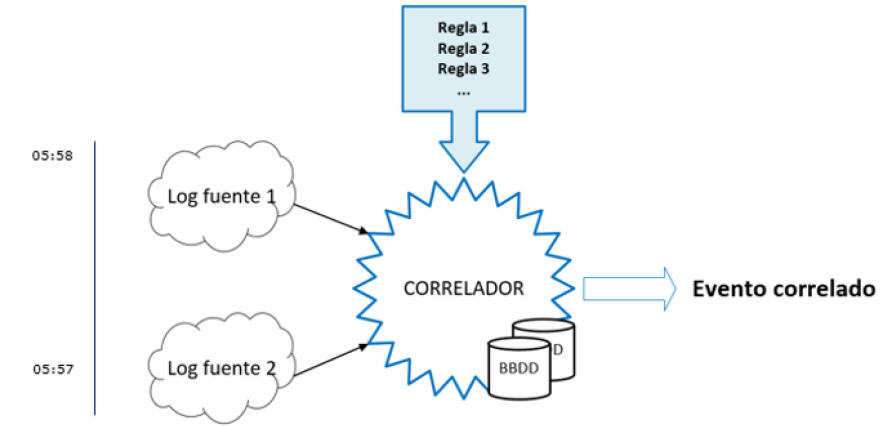
\includegraphics[scale=0.5]{./imagenes/correlado}
    \caption{Esquema de un evento correlado}
\end{figure}\\

La correlación de eventos es útil en distintos escenarios, como el análisis de datos financieros o detección de fraude. Por ejemplo, detectar los patrones de uso infrecuente de una tarjeta de crédito nos permitiría ver ese posible fraude. Por otro lado, podemos utilizarlo para el análisis de logs de un sistema, agrupando eventos y mensajes similares o análisis de gestión y sistemas.\\

Por otro lado, hablaremos de \textbf{agregación o eventos agregados} cuando se agrupen aquellos eventos de la misma tipología, que compartan ciertos campos con idéntico valor, recibidos en un periodo de tiempo \textit{t} definido, con el fin de reducir el número de eventos recibidos. Estos campos son generalmente configurables por el administrador de la plataforma SIEM, así como la propia agregación puede ser deshabilitada si así se desea. La agregación de eventos proporciona soluciones para la administración de logs desde múltiples fuentes, incluyendo aplicaciones, redes, servidores o bases de datos, proporcionando la capacidad de consolidar y agrupar los datos estudiados, para evitar la pérdida de los eventos cruciales. \\ 
\begin{figure}[h]
    \centering
    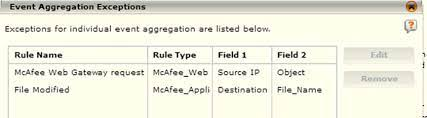
\includegraphics[scale=0.7]{./imagenes/descarga}
    \caption{Ejemplo de opciones de agregación de McAffe}
\end{figure}\\
Un ejemplo de uso simplista, podría ser que si encontramos múltiples intentos de inicio de sesión de un usuario específico fallidos debido a una contraseña incorrecta,  puede reflejarse en un sólo evento de "autenticación fallida" que incluye varios duplicados.





% -------------------------------------------------% -------------------------------------------------
\subsubsection*{¿Se emplean siempre los mismos criterios de agregación en todos los eventos o tipologías de eventos que se reciben en un SIEM? ¿Por qué? Justifique y razone su respuesta de acuerdo a eventos concretos o tipologías de eventos concretas.}

En general, no considero que se empleen los mismos criterios de agregación en los eventos o tipologías, ya que cada sistema generará unos eventos distintos y estos habrán de ser tratados de manera distinta. Según la configuración que tengan esos eventos, habrán de ser tratados y filtrados de forma diferente.\\
Pongamos como ejemplo los eventos que sirven apra monitorizar el rendimiento del sistema, o si la seguridad del mismo está comprometida, no serán tratados de la misma forma. Además, no todos los SIEM ofertarán las mismas características de agregación pues sabemos que \textit{Splunk} a día de hoy no tiene agregación.\\
También hemos de tener en cuenta criterios como la capacidad de almacenamiento (generamos MUCHOS eventos sin ni siquiera saberlo) de nuestros sistemas, factores económicos (pues a mayor cantidad de datos, mayor la inversión que hemos de hacer) o que Windows y Linux no van a generar los mismos eventos. 

% -------------------------------------------------% -------------------------------------------------
\subsubsection*{Durante el curso, hemos estudiado los tipos de visualizaciones que se pueden utilizar para diferentes casuísticas (Compliance, Estado). Si quisiéramos hacer un panel en el que se desea representar gráficamente la evolución de eventos de dos fuentes de datos en un mismo periodo de tiempo, ¿cuál sería la gráfica que utilizaría para dicho fin? Justifique su elección.}

Para este caso utilizaría un dashboard con gráficos de distribución pues nos permite visualizar de mejor manera la evolución de los eventos en distintas fuentes de datos en un mismo periodo de tiempo. Además de permitir ver la información resumida de forma visual, permite que la visualización sea en un espacio temporal determinado por el usuario.\\ 
Adjunto también un diagrama para saber qué representación suele ser la más adecuada para qué tipo de datos y casos.

\begin{figure}[h]
    \centering
    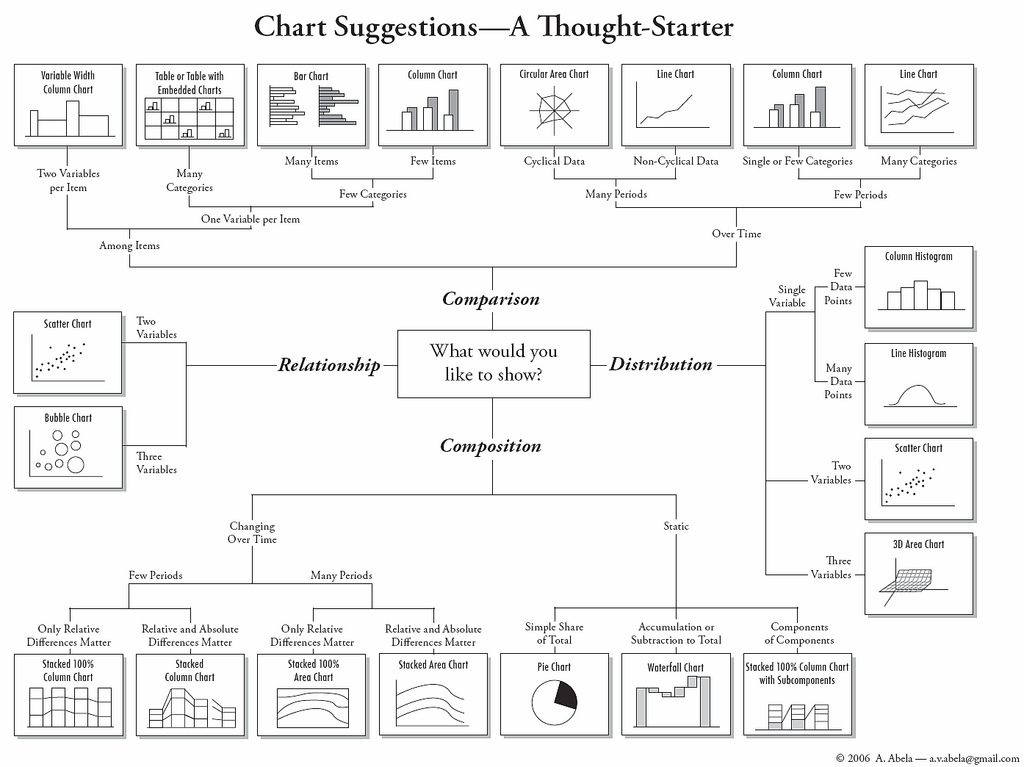
\includegraphics[scale=0.4]{./imagenes/VB2010-01-29A}
    \caption{Criterios para charts}
\end{figure}\\



% -------------------------------------------------% -------------------------------------------------
\subsubsection*{Durante el curso, hemos estudiado los tipos de visualizaciones que se pueden utilizar para diferentes casuísticas (Compliance, Estado). Si quisiéramos hacer una visualización de los eventos tal cual, ¿cuál sería la gráfica o el tipo de visualización para mostrar estos datos? Justifique su respuesta.}

Aparentemente un dashboard sería la mejor opción visual, pero nos obligaría a tratar los datos y no nos sirve (ya que el enunciado dice que queremos los eventos "tal cual"), entonces una tabla de datos es la solución adecuada. 

\end{document} 

